% Fancy arrows drawn with the PGF 3.0 arrows.meta library
% Author: Qrrbrbirlbel
\documentclass[tikz,border=10pt]{standalone}
%%%<
\usepackage{verbatim}
%%%>
\begin{comment}
:Title: Fancy arrows drawn with the PGF 3.0 arrows.meta library
:Tags: Arrows;Decorations;Styles;PGF 3.0
:Author: Qrrbrbirlbel
:Slug: fancy-arrows

PGF 3.0 provides a new library called arrows.meta. Now you can bend arrows,
change arrow tips on the fly, have several arrow tips in a row, and you can use
a special syntax for changing the individual appearance.
You can scale, color, joing, bend, flex, and more, and now there are
a lot of more predefined arrow tips.

This code was written by Qrrbrbirlbel and published on TeX.SE.
\end{comment}
\usetikzlibrary{shapes.geometric,arrows.meta,decorations.markings}
\tikzset{
  big dot/.style={circle, draw, inner sep=0pt, minimum size=3mm, fill=yellow},
  input/.style={draw, trapezium, trapezium left angle=60, trapezium right angle=120,
    line width=1.2pt, fill={rgb:black,1;white,2}},
  obstacle/.style={draw, trapezium, trapezium left angle=120, trapezium right angle=60,
    line width=1.2pt, fill={rgb:black,1;white,2}},
  flash/.style args={#1:#2}{postaction=decorate,decoration={name=markings,
    mark=at position #1 with {%
    \draw[fill=#2, line width=.75\pgflinewidth, line cap=round, line join=round]
         (+\pgflinewidth,+7\pgflinewidth)   -- ++ ( left:+2\pgflinewidth) 
      -- (+-4\pgflinewidth,+-\pgflinewidth) -- ++ (right:+5\pgflinewidth)
      -- (+-\pgflinewidth,+-7\pgflinewidth) -- ++ (right:+2\pgflinewidth)
      -- (+4\pgflinewidth,\pgflinewidth)    -- ++ (left:+5\pgflinewidth)
      -- cycle;}}}
}
\begin{document}
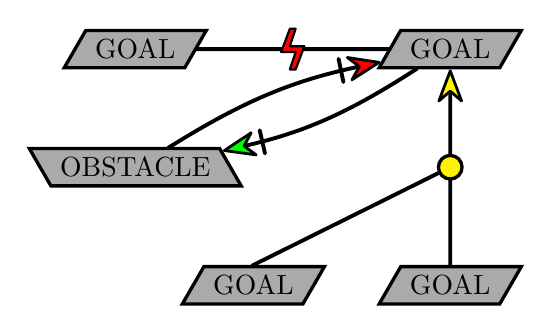
\begin{tikzpicture}[very thick,
  StealthFill/.tip={Stealth[line width=1pt, scale=1.5]}, arrows={[round]}]
\node[input]    (goal1)     at (0,0) {GOAL};
\node[input]    (goal2)     at (4,0) {GOAL};
\node[obstacle] (obstacle1) at (0,-1.5) {OBSTACLE};
\node[input]    (goal3)     at (1.5,-3) {GOAL};
\node[input]    (goal4)     at (4,-3) {GOAL};

\path (goal2) -- node[big dot] (bigdot) {} (goal4);
\path[line width=1.4pt, line cap=rect]
  (goal1) edge[flash=.5:red] (goal2)
  (bigdot) edge (goal3.north)
           edge (goal4)          
           edge[-{StealthFill[fill=yellow]}] (goal2)
  [bend left=10, StealthBar/.style={-{Bar[sep=2] StealthFill[fill=#1]}}]
    (goal2)     edge[StealthBar=green] (obstacle1)
    (obstacle1) edge[StealthBar=red]   (goal2);
\end{tikzpicture}
\end{document}